\documentclass{standalone}
\usepackage{tikz}
\usepackage{ctex,siunitx}
\usepackage{tkz-euclide}
\usepackage{amsmath}
\usetikzlibrary{patterns, calc}
\usetikzlibrary {decorations.pathmorphing, decorations.pathreplacing, decorations.shapes,}
\begin{document}
\small
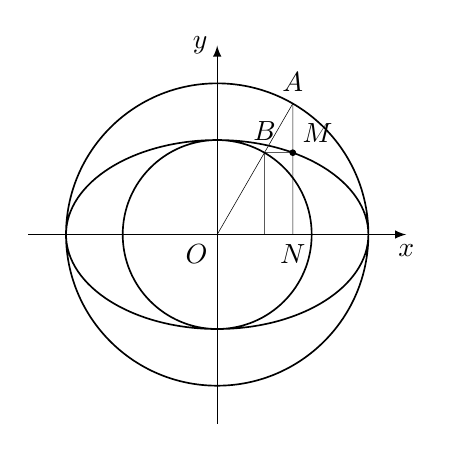
\begin{tikzpicture}[>=latex,scale=1.2]
  \tkzDefPoints{0/0/O,1/0/x,0/1/y}
  \tkzDefPoint(60:1.6){A}
  \tkzDefPoint(60:1.0){B}
  \tkzDefPointsBy[projection=onto O--x](A,B){N,P}
  \tkzDefPointsBy[projection=onto A--N](B){M}
  \draw[thin,->](-2,0)--(2,0)node[below]{$x$};
  \draw[thin,->](0,-2)--(0,2)node[left]{$y$};
  \draw [semithick](O) circle (1.6)(O) circle (1.0)(O) ellipse (1.6 and 1.0);
  \tkzDrawSegments(A,N B,M B,P O,A)
  \tkzDrawPoints[fill=black](M)
  \tkzLabelPoints[below left](O)
  \tkzLabelPoints[below](N)
  \tkzLabelPoints[above=1pt](A,B)
  \tkzLabelPoints[above right](M)
  % \tkzLabelPoints[above left](B)
\end{tikzpicture}
\end{document}